% Options for packages loaded elsewhere
\PassOptionsToPackage{unicode}{hyperref}
\PassOptionsToPackage{hyphens}{url}
\PassOptionsToPackage{dvipsnames,svgnames,x11names}{xcolor}
%
\documentclass[
  letterpaper,
  DIV=11,
  numbers=noendperiod]{scrartcl}

\usepackage{amsmath,amssymb}
\usepackage{iftex}
\ifPDFTeX
  \usepackage[T1]{fontenc}
  \usepackage[utf8]{inputenc}
  \usepackage{textcomp} % provide euro and other symbols
\else % if luatex or xetex
  \usepackage{unicode-math}
  \defaultfontfeatures{Scale=MatchLowercase}
  \defaultfontfeatures[\rmfamily]{Ligatures=TeX,Scale=1}
\fi
\usepackage{lmodern}
\ifPDFTeX\else  
    % xetex/luatex font selection
\fi
% Use upquote if available, for straight quotes in verbatim environments
\IfFileExists{upquote.sty}{\usepackage{upquote}}{}
\IfFileExists{microtype.sty}{% use microtype if available
  \usepackage[]{microtype}
  \UseMicrotypeSet[protrusion]{basicmath} % disable protrusion for tt fonts
}{}
\makeatletter
\@ifundefined{KOMAClassName}{% if non-KOMA class
  \IfFileExists{parskip.sty}{%
    \usepackage{parskip}
  }{% else
    \setlength{\parindent}{0pt}
    \setlength{\parskip}{6pt plus 2pt minus 1pt}}
}{% if KOMA class
  \KOMAoptions{parskip=half}}
\makeatother
\usepackage{xcolor}
\setlength{\emergencystretch}{3em} % prevent overfull lines
\setcounter{secnumdepth}{5}
% Make \paragraph and \subparagraph free-standing
\ifx\paragraph\undefined\else
  \let\oldparagraph\paragraph
  \renewcommand{\paragraph}[1]{\oldparagraph{#1}\mbox{}}
\fi
\ifx\subparagraph\undefined\else
  \let\oldsubparagraph\subparagraph
  \renewcommand{\subparagraph}[1]{\oldsubparagraph{#1}\mbox{}}
\fi

\usepackage{color}
\usepackage{fancyvrb}
\newcommand{\VerbBar}{|}
\newcommand{\VERB}{\Verb[commandchars=\\\{\}]}
\DefineVerbatimEnvironment{Highlighting}{Verbatim}{commandchars=\\\{\}}
% Add ',fontsize=\small' for more characters per line
\usepackage{framed}
\definecolor{shadecolor}{RGB}{241,243,245}
\newenvironment{Shaded}{\begin{snugshade}}{\end{snugshade}}
\newcommand{\AlertTok}[1]{\textcolor[rgb]{0.68,0.00,0.00}{#1}}
\newcommand{\AnnotationTok}[1]{\textcolor[rgb]{0.37,0.37,0.37}{#1}}
\newcommand{\AttributeTok}[1]{\textcolor[rgb]{0.40,0.45,0.13}{#1}}
\newcommand{\BaseNTok}[1]{\textcolor[rgb]{0.68,0.00,0.00}{#1}}
\newcommand{\BuiltInTok}[1]{\textcolor[rgb]{0.00,0.23,0.31}{#1}}
\newcommand{\CharTok}[1]{\textcolor[rgb]{0.13,0.47,0.30}{#1}}
\newcommand{\CommentTok}[1]{\textcolor[rgb]{0.37,0.37,0.37}{#1}}
\newcommand{\CommentVarTok}[1]{\textcolor[rgb]{0.37,0.37,0.37}{\textit{#1}}}
\newcommand{\ConstantTok}[1]{\textcolor[rgb]{0.56,0.35,0.01}{#1}}
\newcommand{\ControlFlowTok}[1]{\textcolor[rgb]{0.00,0.23,0.31}{#1}}
\newcommand{\DataTypeTok}[1]{\textcolor[rgb]{0.68,0.00,0.00}{#1}}
\newcommand{\DecValTok}[1]{\textcolor[rgb]{0.68,0.00,0.00}{#1}}
\newcommand{\DocumentationTok}[1]{\textcolor[rgb]{0.37,0.37,0.37}{\textit{#1}}}
\newcommand{\ErrorTok}[1]{\textcolor[rgb]{0.68,0.00,0.00}{#1}}
\newcommand{\ExtensionTok}[1]{\textcolor[rgb]{0.00,0.23,0.31}{#1}}
\newcommand{\FloatTok}[1]{\textcolor[rgb]{0.68,0.00,0.00}{#1}}
\newcommand{\FunctionTok}[1]{\textcolor[rgb]{0.28,0.35,0.67}{#1}}
\newcommand{\ImportTok}[1]{\textcolor[rgb]{0.00,0.46,0.62}{#1}}
\newcommand{\InformationTok}[1]{\textcolor[rgb]{0.37,0.37,0.37}{#1}}
\newcommand{\KeywordTok}[1]{\textcolor[rgb]{0.00,0.23,0.31}{#1}}
\newcommand{\NormalTok}[1]{\textcolor[rgb]{0.00,0.23,0.31}{#1}}
\newcommand{\OperatorTok}[1]{\textcolor[rgb]{0.37,0.37,0.37}{#1}}
\newcommand{\OtherTok}[1]{\textcolor[rgb]{0.00,0.23,0.31}{#1}}
\newcommand{\PreprocessorTok}[1]{\textcolor[rgb]{0.68,0.00,0.00}{#1}}
\newcommand{\RegionMarkerTok}[1]{\textcolor[rgb]{0.00,0.23,0.31}{#1}}
\newcommand{\SpecialCharTok}[1]{\textcolor[rgb]{0.37,0.37,0.37}{#1}}
\newcommand{\SpecialStringTok}[1]{\textcolor[rgb]{0.13,0.47,0.30}{#1}}
\newcommand{\StringTok}[1]{\textcolor[rgb]{0.13,0.47,0.30}{#1}}
\newcommand{\VariableTok}[1]{\textcolor[rgb]{0.07,0.07,0.07}{#1}}
\newcommand{\VerbatimStringTok}[1]{\textcolor[rgb]{0.13,0.47,0.30}{#1}}
\newcommand{\WarningTok}[1]{\textcolor[rgb]{0.37,0.37,0.37}{\textit{#1}}}

\providecommand{\tightlist}{%
  \setlength{\itemsep}{0pt}\setlength{\parskip}{0pt}}\usepackage{longtable,booktabs,array}
\usepackage{calc} % for calculating minipage widths
% Correct order of tables after \paragraph or \subparagraph
\usepackage{etoolbox}
\makeatletter
\patchcmd\longtable{\par}{\if@noskipsec\mbox{}\fi\par}{}{}
\makeatother
% Allow footnotes in longtable head/foot
\IfFileExists{footnotehyper.sty}{\usepackage{footnotehyper}}{\usepackage{footnote}}
\makesavenoteenv{longtable}
\usepackage{graphicx}
\makeatletter
\def\maxwidth{\ifdim\Gin@nat@width>\linewidth\linewidth\else\Gin@nat@width\fi}
\def\maxheight{\ifdim\Gin@nat@height>\textheight\textheight\else\Gin@nat@height\fi}
\makeatother
% Scale images if necessary, so that they will not overflow the page
% margins by default, and it is still possible to overwrite the defaults
% using explicit options in \includegraphics[width, height, ...]{}
\setkeys{Gin}{width=\maxwidth,height=\maxheight,keepaspectratio}
% Set default figure placement to htbp
\makeatletter
\def\fps@figure{htbp}
\makeatother

\KOMAoption{captions}{tableheading}
\makeatletter
\makeatother
\makeatletter
\makeatother
\makeatletter
\@ifpackageloaded{caption}{}{\usepackage{caption}}
\AtBeginDocument{%
\ifdefined\contentsname
  \renewcommand*\contentsname{Table of contents}
\else
  \newcommand\contentsname{Table of contents}
\fi
\ifdefined\listfigurename
  \renewcommand*\listfigurename{List of Figures}
\else
  \newcommand\listfigurename{List of Figures}
\fi
\ifdefined\listtablename
  \renewcommand*\listtablename{List of Tables}
\else
  \newcommand\listtablename{List of Tables}
\fi
\ifdefined\figurename
  \renewcommand*\figurename{Figure}
\else
  \newcommand\figurename{Figure}
\fi
\ifdefined\tablename
  \renewcommand*\tablename{Table}
\else
  \newcommand\tablename{Table}
\fi
}
\@ifpackageloaded{float}{}{\usepackage{float}}
\floatstyle{ruled}
\@ifundefined{c@chapter}{\newfloat{codelisting}{h}{lop}}{\newfloat{codelisting}{h}{lop}[chapter]}
\floatname{codelisting}{Listing}
\newcommand*\listoflistings{\listof{codelisting}{List of Listings}}
\makeatother
\makeatletter
\@ifpackageloaded{caption}{}{\usepackage{caption}}
\@ifpackageloaded{subcaption}{}{\usepackage{subcaption}}
\makeatother
\makeatletter
\@ifpackageloaded{tcolorbox}{}{\usepackage[skins,breakable]{tcolorbox}}
\makeatother
\makeatletter
\@ifundefined{shadecolor}{\definecolor{shadecolor}{rgb}{.97, .97, .97}}
\makeatother
\makeatletter
\makeatother
\makeatletter
\makeatother
\ifLuaTeX
  \usepackage{selnolig}  % disable illegal ligatures
\fi
\IfFileExists{bookmark.sty}{\usepackage{bookmark}}{\usepackage{hyperref}}
\IfFileExists{xurl.sty}{\usepackage{xurl}}{} % add URL line breaks if available
\urlstyle{same} % disable monospaced font for URLs
\hypersetup{
  pdftitle={Overview of the Quantitative Histories Workshop},
  pdfauthor={Howard University},
  colorlinks=true,
  linkcolor={blue},
  filecolor={Maroon},
  citecolor={Blue},
  urlcolor={Blue},
  pdfcreator={LaTeX via pandoc}}

\title{Overview of the Quantitative Histories Workshop}
\usepackage{etoolbox}
\makeatletter
\providecommand{\subtitle}[1]{% add subtitle to \maketitle
  \apptocmd{\@title}{\par {\large #1 \par}}{}{}
}
\makeatother
\subtitle{Nathan Alexander, Ph.D.}
\author{Howard University}
\date{}

\begin{document}
\maketitle
\ifdefined\Shaded\renewenvironment{Shaded}{\begin{tcolorbox}[boxrule=0pt, sharp corners, breakable, interior hidden, frame hidden, borderline west={3pt}{0pt}{shadecolor}, enhanced]}{\end{tcolorbox}}\fi

\renewcommand*\contentsname{Table of contents}
{
\hypersetup{linkcolor=}
\setcounter{tocdepth}{3}
\tableofcontents
}
\hypertarget{quantitative-histories-workshop}{%
\section{Quantitative Histories
Workshop}\label{quantitative-histories-workshop}}

\texttt{Curriculum\ \&\ software\ development\ collective}

and

{research lab}

\hypertarget{research-problem}{%
\section{Research Problem}\label{research-problem}}

{Increasingly complex problems require complex tools.}

Computational tools support interdisciplinary thinking.

\hypertarget{research-problem-1}{%
\section{Research Problem}\label{research-problem-1}}

Increasingly complex problems require complex tools.

{Computational tools support interdisciplinary thinking.}

\hypertarget{research-problem-2}{%
\section{Research Problem}\label{research-problem-2}}

Increasingly complex problems require complex tools.

Sub-disciplinary tools require interdisciplinary thinking.

{How can information theory inform interdisciplinary curriculum and
software development?}

\hypertarget{information-theory}{%
\section{Information theory}\label{information-theory}}

Information theory is a branch of applied mathematics and computer
science that deals with the quantification, storage, transmission, and
manipulation of information. We take an abstract approach to our study
of information.

\begin{itemize}
\item
  Information theory seeks to measure the amount of information
  contained in a \emph{message} or signal and how efficiently it can be
  transmitted or stored.
\item
  In this way, our projects define \emph{information} using a curricular
  perspective.
\end{itemize}

\hypertarget{quantitative-history}{%
\section{Quantitative history}\label{quantitative-history}}

\begin{figure}

{\centering 
\includegraphics[width=0.5\textwidth,height=\textheight]{quanthist.jpg}

}

\caption{\emph{Historie Quantitative} by Pierre Chaunu}

\end{figure}

\hypertarget{mathematical-sociology}{%
\section{Mathematical sociology}\label{mathematical-sociology}}

\begin{figure}

{\centering 
\includegraphics[width=0.5\textwidth,height=\textheight]{math-soc.jpg}

}

\caption{\emph{Journal of Mathematical Sociology}}

\end{figure}

\hypertarget{curriculum-and-software-development}{%
\section{Curriculum and software
development}\label{curriculum-and-software-development}}

Design, development, implementation, and evaluation of computational
curricular materials

\hypertarget{research-projects}{%
\subsection{Research projects}\label{research-projects}}

\begin{itemize}
\item
  ECHO: Education, Community, and Health Observations

  \begin{itemize}
  \tightlist
  \item
    Information and spatial segregation
  \end{itemize}
\item
  Teaching statistical learning and mathematical modeling
\item
  Theory and quantification
\end{itemize}

\begin{center}\rule{0.5\linewidth}{0.5pt}\end{center}

\hypertarget{project-group-1-spatial-information-and-racial-isolation}{%
\subsection{Project group 1: Spatial information and racial
isolation}\label{project-group-1-spatial-information-and-racial-isolation}}

How do patterns of racial segregation inform education, community, and
health outcomes?

\begin{itemize}
\item
  Historical legacies of injustice
\item
  Traditional modeling approaches
\item
  Modern computational tools
\end{itemize}

\hypertarget{dividing-walls}{%
\section{Dividing walls}\label{dividing-walls}}

\hypertarget{geometric-approach}{%
\section{Geometric approach}\label{geometric-approach}}

We adopt a \textbf{topological} model for spatial segregation on a
geographical area, \(G\) to develop a theory of dividing walls.

Builds on the topological and topographical work of Short (2011).

\textbf{Theorem 1}. Given any configuration of blue and green towns,
there is a dividing wall that separates blue towns from green towns.

\begin{figure}

{\centering 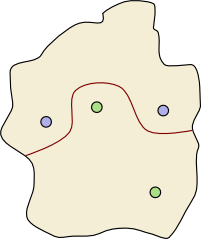
\includegraphics[width=0.5\textwidth,height=\textheight]{wall-2.png}

}

\caption{Geographic area with neighborhood units}

\end{figure}

\begin{center}\rule{0.5\linewidth}{0.5pt}\end{center}

\textbf{Theorem 1}. Given any configuration of blue and green towns,
there is a dividing wall that separates blue towns from green towns.

\begin{figure}

{\centering 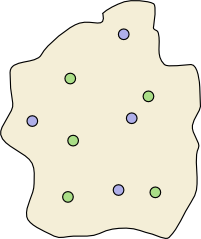
\includegraphics[width=0.5\textwidth,height=\textheight]{wall-1.png}

}

\caption{Geographic area with neighborhood units}

\end{figure}

\begin{center}\rule{0.5\linewidth}{0.5pt}\end{center}

\textbf{Theorem 1}. Given any configuration of blue and green towns,
there is a dividing wall that separates blue towns from green towns.

\begin{figure}

{\centering 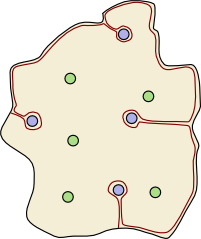
\includegraphics[width=0.5\textwidth,height=\textheight]{wall-0.png}

}

\caption{Geographic area with wall dividing neighborhood units}

\end{figure}

\begin{center}\rule{0.5\linewidth}{0.5pt}\end{center}

\hypertarget{is-there-a-dividing-wall-for-an-island-with-coastal-towns}{%
\subsection{Is there a dividing wall for an island with coastal
towns?}\label{is-there-a-dividing-wall-for-an-island-with-coastal-towns}}

\begin{figure}

{\centering 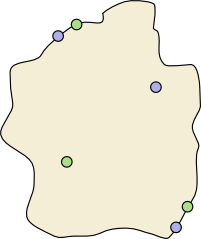
\includegraphics[width=0.5\textwidth,height=\textheight]{wall-3.png}

}

\caption{Island with coastal towns}

\end{figure}

\begin{center}\rule{0.5\linewidth}{0.5pt}\end{center}

\hypertarget{is-there-a-dividing-wall-for-an-island-with-coastal-towns-1}{%
\subsection{Is there a dividing wall for an island with coastal
towns?}\label{is-there-a-dividing-wall-for-an-island-with-coastal-towns-1}}

\begin{figure}

{\centering 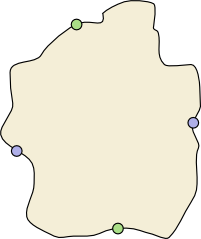
\includegraphics[width=0.5\textwidth,height=\textheight]{wall-4.png}

}

\caption{Minimal configuration}

\end{figure}

\begin{center}\rule{0.5\linewidth}{0.5pt}\end{center}

\begin{figure}

{\centering 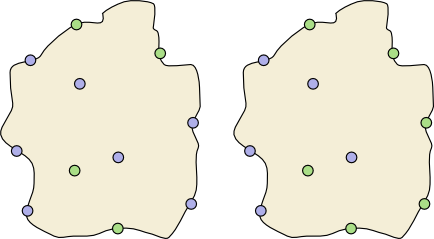
\includegraphics[width=0.5\textwidth,height=\textheight]{wall-5.png}

}

\caption{Alternating configuration (left) and non-alternating
configuration (right).}

\end{figure}

\textbf{Theorem 2}. Alternating configurations of towns do not have a
dividing wall, whereas non-alternating configurations of towns do have a
dividing wall.

\begin{center}\rule{0.5\linewidth}{0.5pt}\end{center}

\hypertarget{algebraic-approach}{%
\subsubsection{Algebraic approach}\label{algebraic-approach}}

We then develop a algebraic modeling approach using methods from
\textbf{mathematical sociology}.

Segregation indices

\begin{itemize}
\item
  \emph{Dissimilarity index}: Measures the proportion of one group's
  population that would need to move to achieve an even distribution
  across all areas. It ranges from 0 to 1, with higher values indicating
  greater segregation.
\item
  \emph{Isolation index}: Measures the extent to which members of a
  particular group are surrounded by others from the same group. It
  represents the percentage of people from a specific group who would
  need to change neighborhoods to achieve an even distribution. Higher
  values indicate higher isolation and segregation.
\end{itemize}

\begin{center}\rule{0.5\linewidth}{0.5pt}\end{center}

\hypertarget{algebraic-approach-1}{%
\subsubsection{Algebraic approach}\label{algebraic-approach-1}}

We then develop a algebraic modeling approach using methods from
\textbf{mathematical sociology}.

Segregation indices

\begin{itemize}
\item
  \emph{Exposure index}: Measures the extent to which members of one
  group are exposed to members of another group. It quantifies the
  likelihood that a randomly selected individual from one group will
  encounter individuals from another group. Higher values indicate
  higher exposure and lower segregation.
\item
  \emph{Concentration index}: Measures the extent to which a particular
  group is concentrated in specific areas or neighborhoods. It reflects
  the degree of clustering or dispersion of the group's population
  across geographic units.
\item
  \emph{Gini index}: Measure of income inequality, but it can also be
  adapted to measure residential segregation. It provides a summary
  measure of the overall distribution of different groups across
  neighborhoods.
\end{itemize}

\begin{center}\rule{0.5\linewidth}{0.5pt}\end{center}

\hypertarget{index-of-dissimilarity}{%
\subsection{Index of Dissimilarity}\label{index-of-dissimilarity}}

\[ D = \dfrac{1}{2} \sum_\limits{i=1}^n  \bigg| \frac{b_i}{B} - \frac{w_i}{W} \bigg| \]

\begin{itemize}
\item
  \(n\) is the number of neighborhoods in a geographic region,
\item
  \(b_i\) is the number of Black household units in neighborhood \(i\),
\item
  \(B\) is the total number of Black household units in the geographic
  region,
\item
  \(w_i\) is the number of non-Black household units in neighborhood
  \(i\),
\item
  \(W\) is the total number of non-Black household units in the
  geographic region,
\end{itemize}

\begin{center}\rule{0.5\linewidth}{0.5pt}\end{center}

\begin{figure}

{\centering 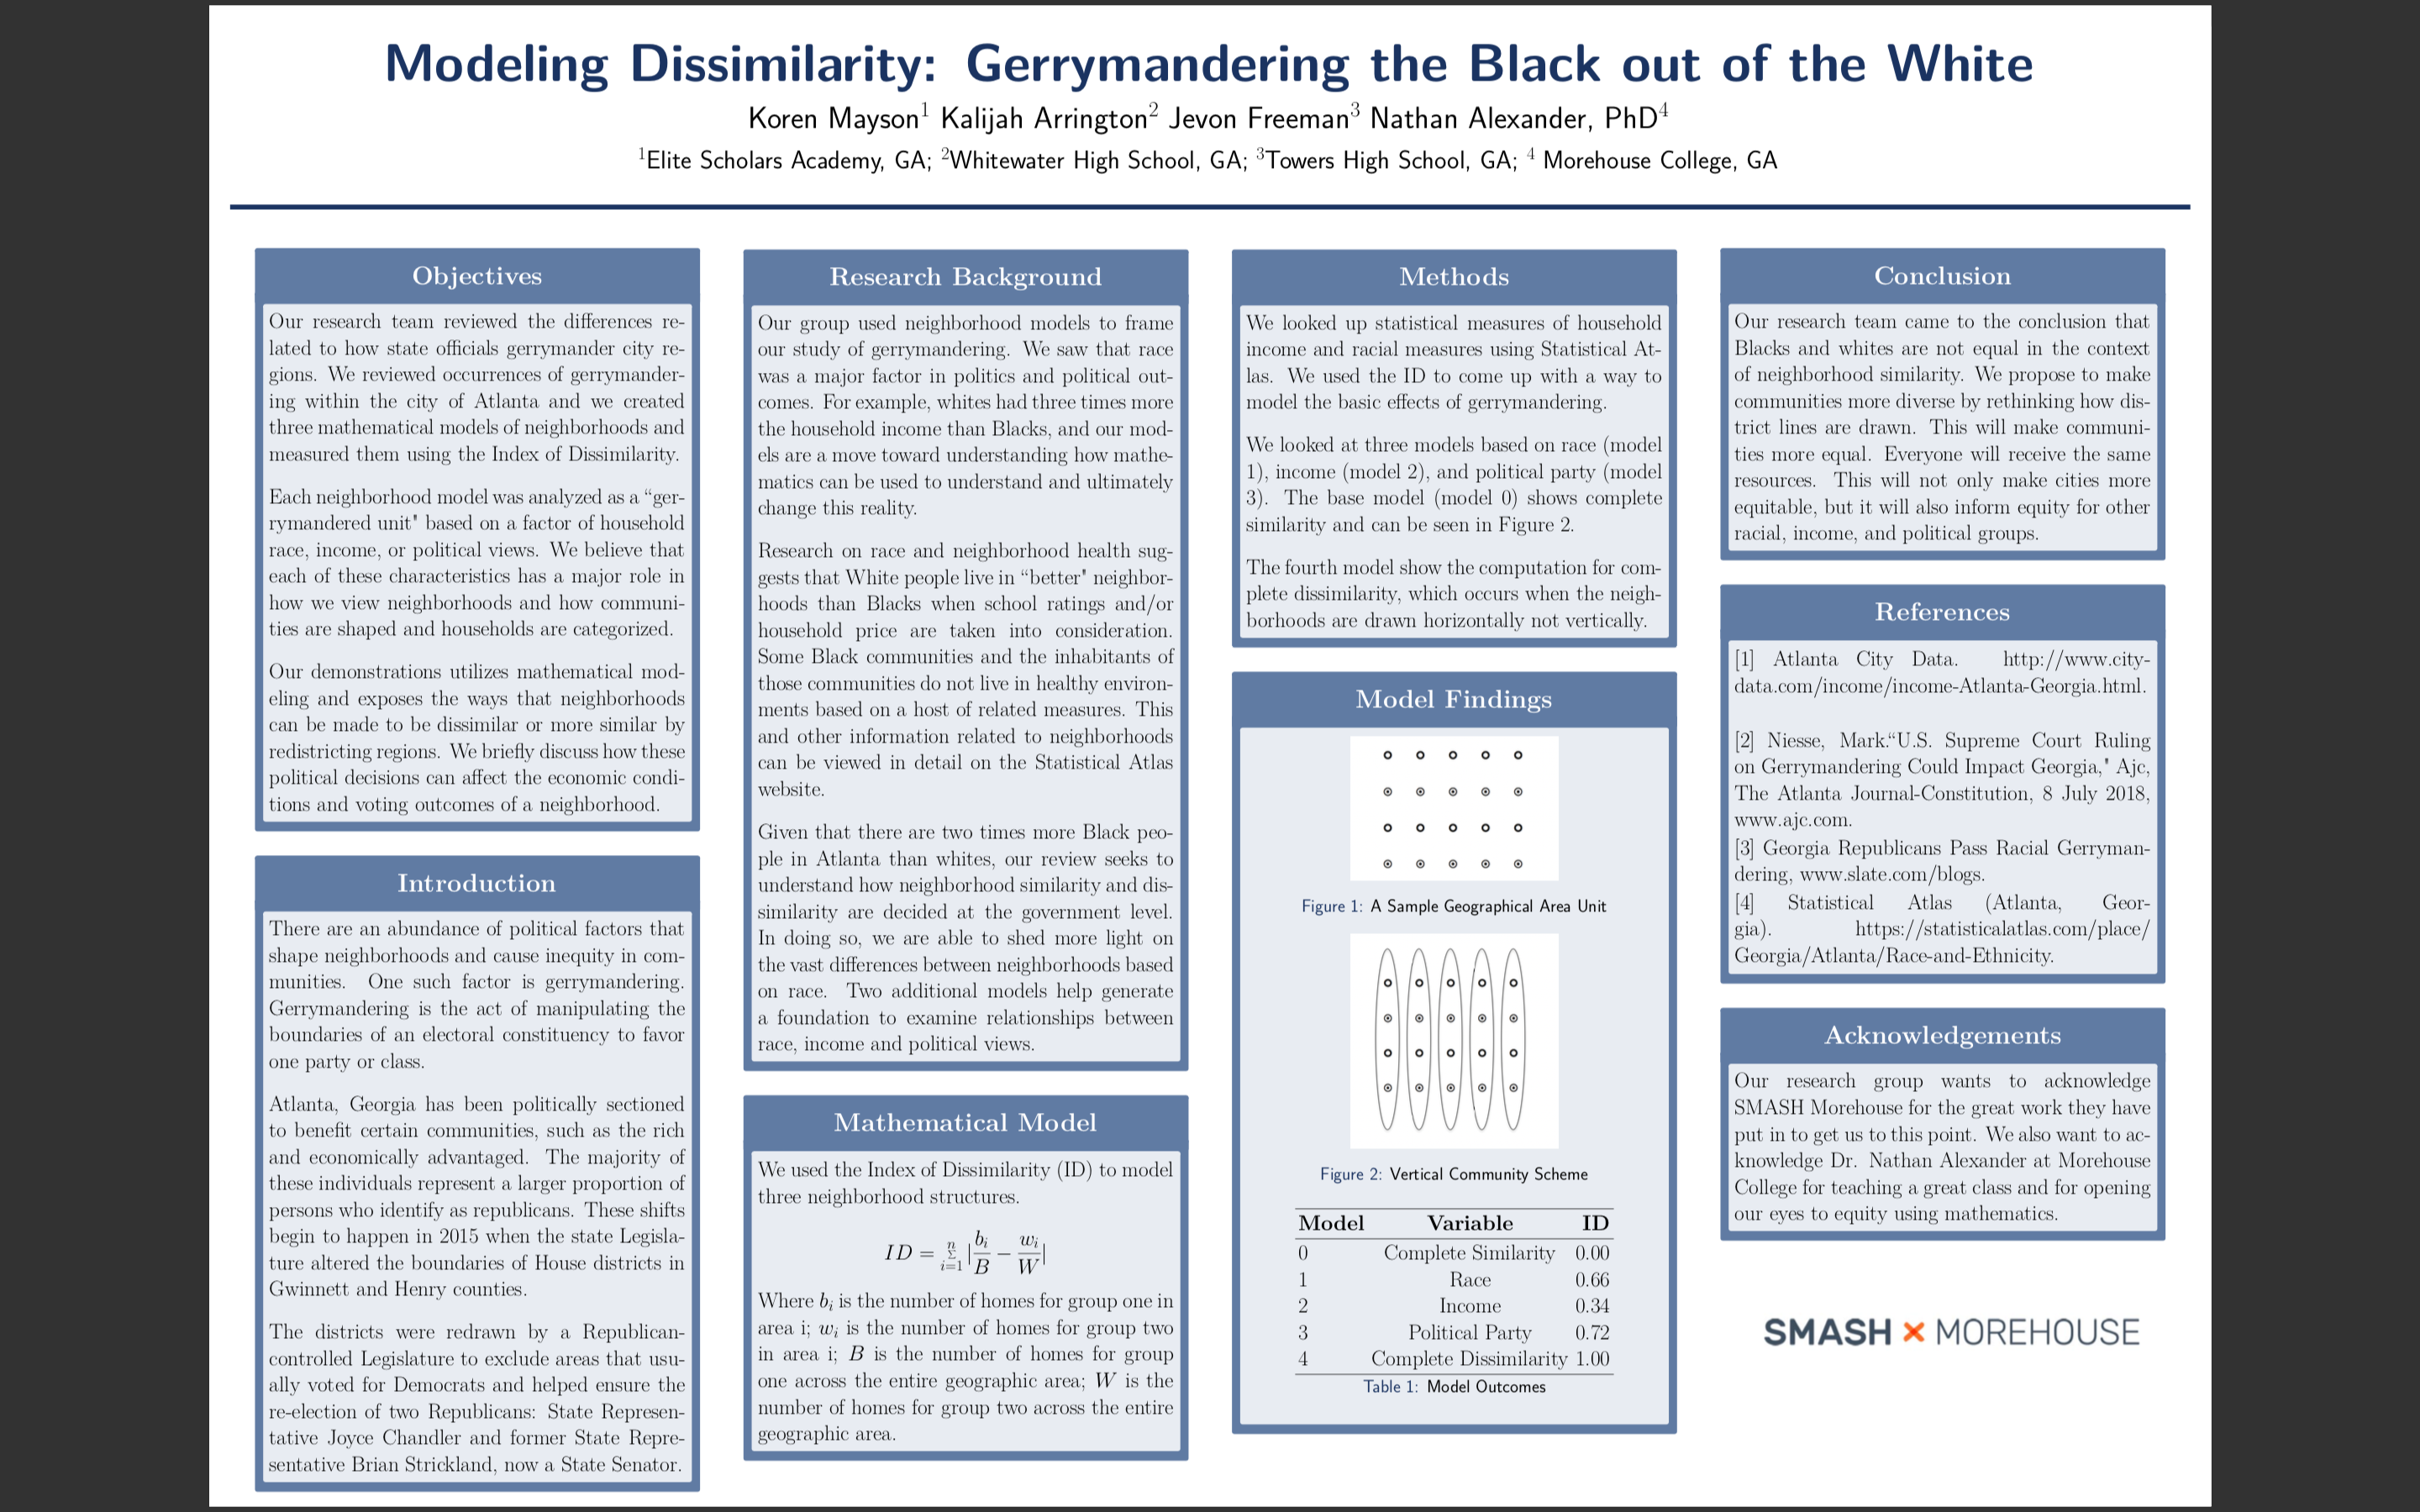
\includegraphics{poster1.png}

}

\caption{Co-authored student research poster.}

\end{figure}

\begin{center}\rule{0.5\linewidth}{0.5pt}\end{center}

\hypertarget{computational-approach}{%
\subsection{Computational approach}\label{computational-approach}}

Teaching computational methods and open source tools makes for efficient
and accurate learning. In about 20 lines of code, there is an immediate
intersection.

\begin{Shaded}
\begin{Highlighting}[]
\NormalTok{black\_georgetown\_sc\_2020 }\OtherTok{\textless{}{-}}
  \FunctionTok{get\_acs}\NormalTok{(}\AttributeTok{geography =} \StringTok{"tract"}\NormalTok{, }\AttributeTok{state =} \StringTok{"SC"}\NormalTok{,}
          \AttributeTok{county =} \StringTok{"Georgetown"}\NormalTok{,}
                        \AttributeTok{variable =} \StringTok{"B02001\_003"}\NormalTok{, }\CommentTok{\# Black or African American Alone}
                        \AttributeTok{geometry =} \ConstantTok{TRUE}\NormalTok{)}
\end{Highlighting}
\end{Shaded}

\begin{verbatim}
Getting data from the 2018-2022 5-year ACS
\end{verbatim}

\begin{verbatim}
Downloading feature geometry from the Census website.  To cache shapefiles for use in future sessions, set `options(tigris_use_cache = TRUE)`.
\end{verbatim}

\begin{verbatim}

  |                                                                            
  |                                                                      |   0%
  |                                                                            
  |=                                                                     |   1%
  |                                                                            
  |==                                                                    |   3%
  |                                                                            
  |===                                                                   |   4%
  |                                                                            
  |===                                                                   |   5%
  |                                                                            
  |====                                                                  |   6%
  |                                                                            
  |=======                                                               |  10%
  |                                                                            
  |==========                                                            |  14%
  |                                                                            
  |============                                                          |  16%
  |                                                                            
  |============                                                          |  18%
  |                                                                            
  |===============                                                       |  22%
  |                                                                            
  |================                                                      |  23%
  |                                                                            
  |==================                                                    |  25%
  |                                                                            
  |======================                                                |  32%
  |                                                                            
  |=========================                                             |  36%
  |                                                                            
  |===============================                                       |  45%
  |                                                                            
  |================================                                      |  46%
  |                                                                            
  |======================================                                |  54%
  |                                                                            
  |======================================                                |  55%
  |                                                                            
  |==============================================                        |  65%
  |                                                                            
  |=====================================================                 |  75%
  |                                                                            
  |=======================================================               |  79%
  |                                                                            
  |==============================================================        |  88%
  |                                                                            
  |===============================================================       |  90%
  |                                                                            
  |================================================================      |  91%
  |                                                                            
  |====================================================================  |  97%
  |                                                                            
  |======================================================================| 100%
\end{verbatim}

\begin{center}\rule{0.5\linewidth}{0.5pt}\end{center}

Estimate of Black or African American alone in Georgetown county, SC.

\begin{verbatim}
Getting data from the 2018-2022 5-year ACS
\end{verbatim}

\begin{verbatim}
Downloading feature geometry from the Census website.  To cache shapefiles for use in future sessions, set `options(tigris_use_cache = TRUE)`.
\end{verbatim}

\begin{verbatim}
Warning in title(...): "title" is not a graphical parameter
\end{verbatim}

\begin{verbatim}
Warning in title(...): "subtitle" is not a graphical parameter
\end{verbatim}

\begin{verbatim}
Warning in title(...): "title" is not a graphical parameter
\end{verbatim}

\begin{verbatim}
Warning in title(...): "subtitle" is not a graphical parameter
\end{verbatim}

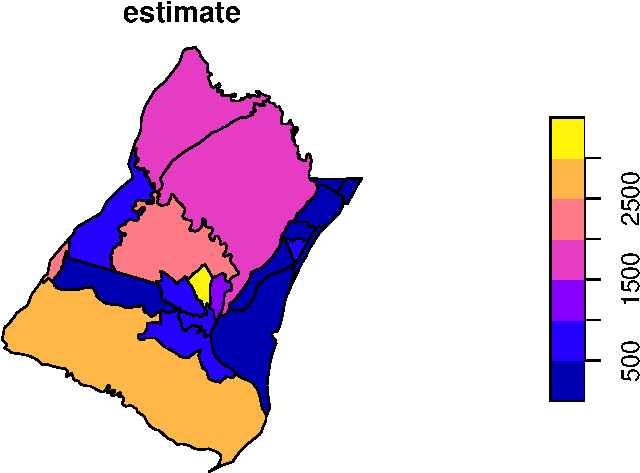
\includegraphics{talk_files/figure-pdf/unnamed-chunk-3-1.pdf}

\hypertarget{historical-and-broader-applications}{%
\section{Historical and broader
applications}\label{historical-and-broader-applications}}

Social politics of maps.

\begin{itemize}
\item
  Introductory module used in graduate course in statistics.
\item
  \texttt{critstats} package developed for students to download and
  explore culturally relevant data.
\end{itemize}

\begin{center}\rule{0.5\linewidth}{0.5pt}\end{center}

\hypertarget{historical-applications}{%
\subsubsection{Historical applications}\label{historical-applications}}

\begin{figure}

{\centering 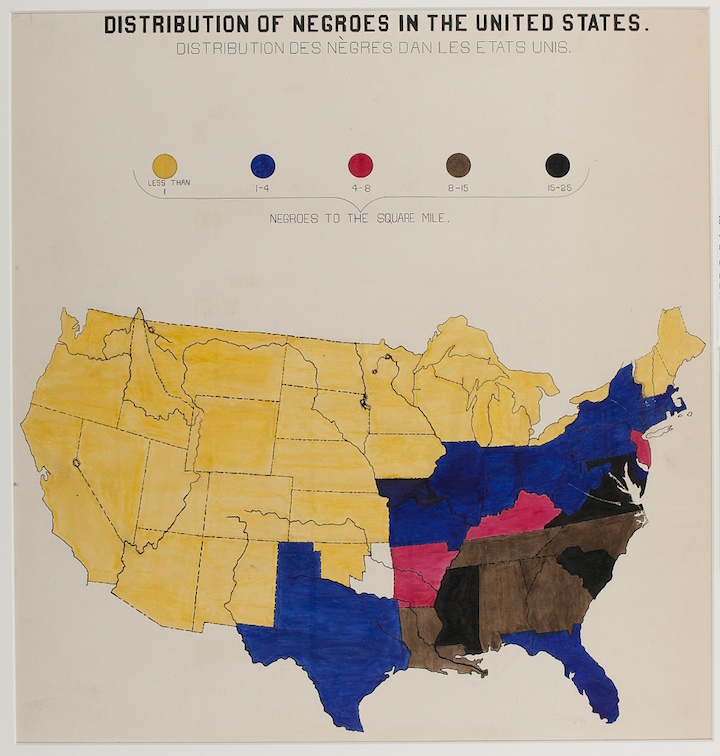
\includegraphics[width=0.5\textwidth,height=\textheight]{w1d2e.jpg}

}

\caption{Distribution of Negroes in the United States.}

\end{figure}

\begin{center}\rule{0.5\linewidth}{0.5pt}\end{center}

\hypertarget{broader-applications}{%
\subsubsection{Broader applications}\label{broader-applications}}

\begin{figure}

{\centering 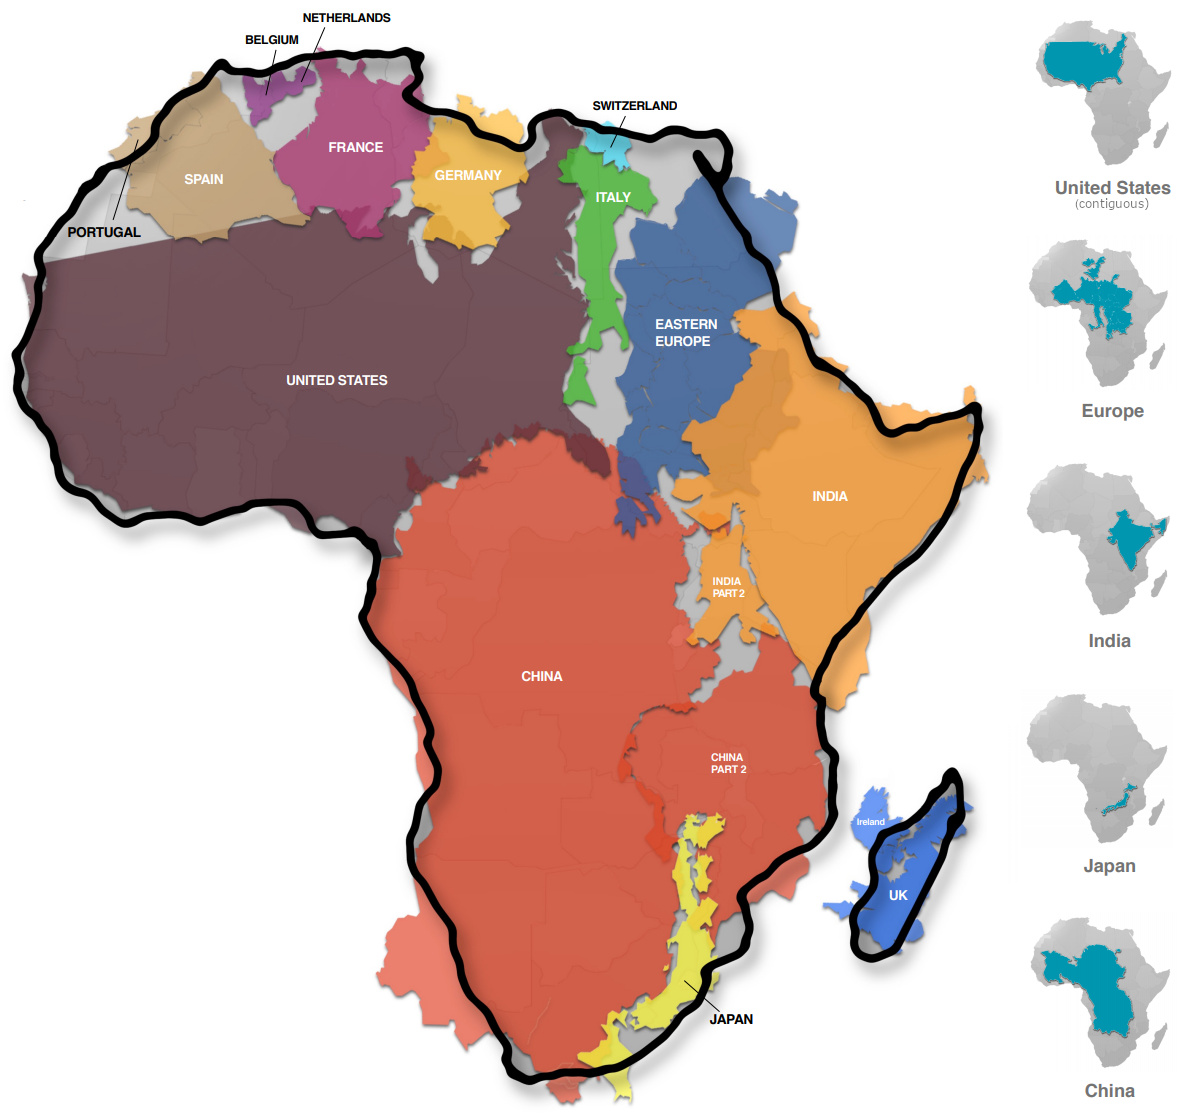
\includegraphics[width=0.5\textwidth,height=\textheight]{true-size-of-africa.jpg}

}

\caption{True Size of Africa.}

\end{figure}

\begin{center}\rule{0.5\linewidth}{0.5pt}\end{center}

\hypertarget{project-group-2-mining-archives-and-historical-text-analysis-of-sentiments-and-textual-data}{%
\subsection{Project group 2: Mining archives and historical text:
Analysis of sentiments and textual
data}\label{project-group-2-mining-archives-and-historical-text-analysis-of-sentiments-and-textual-data}}

\begin{itemize}
\item
  Inquiry into the speeches of historical figures, such as civil rights
  activists.
\item
  Exploration of journal articles and citations related to historical of
  inequity
\end{itemize}

\begin{center}\rule{0.5\linewidth}{0.5pt}\end{center}

\hypertarget{theoretical-foundations-of-sentiment-analysis}{%
\subsubsection{Theoretical foundations of sentiment
analysis}\label{theoretical-foundations-of-sentiment-analysis}}

History, political science, and sociology inform theory development

\begin{figure}

\begin{minipage}[t]{0.50\linewidth}

{\centering 

\raisebox{-\height}{

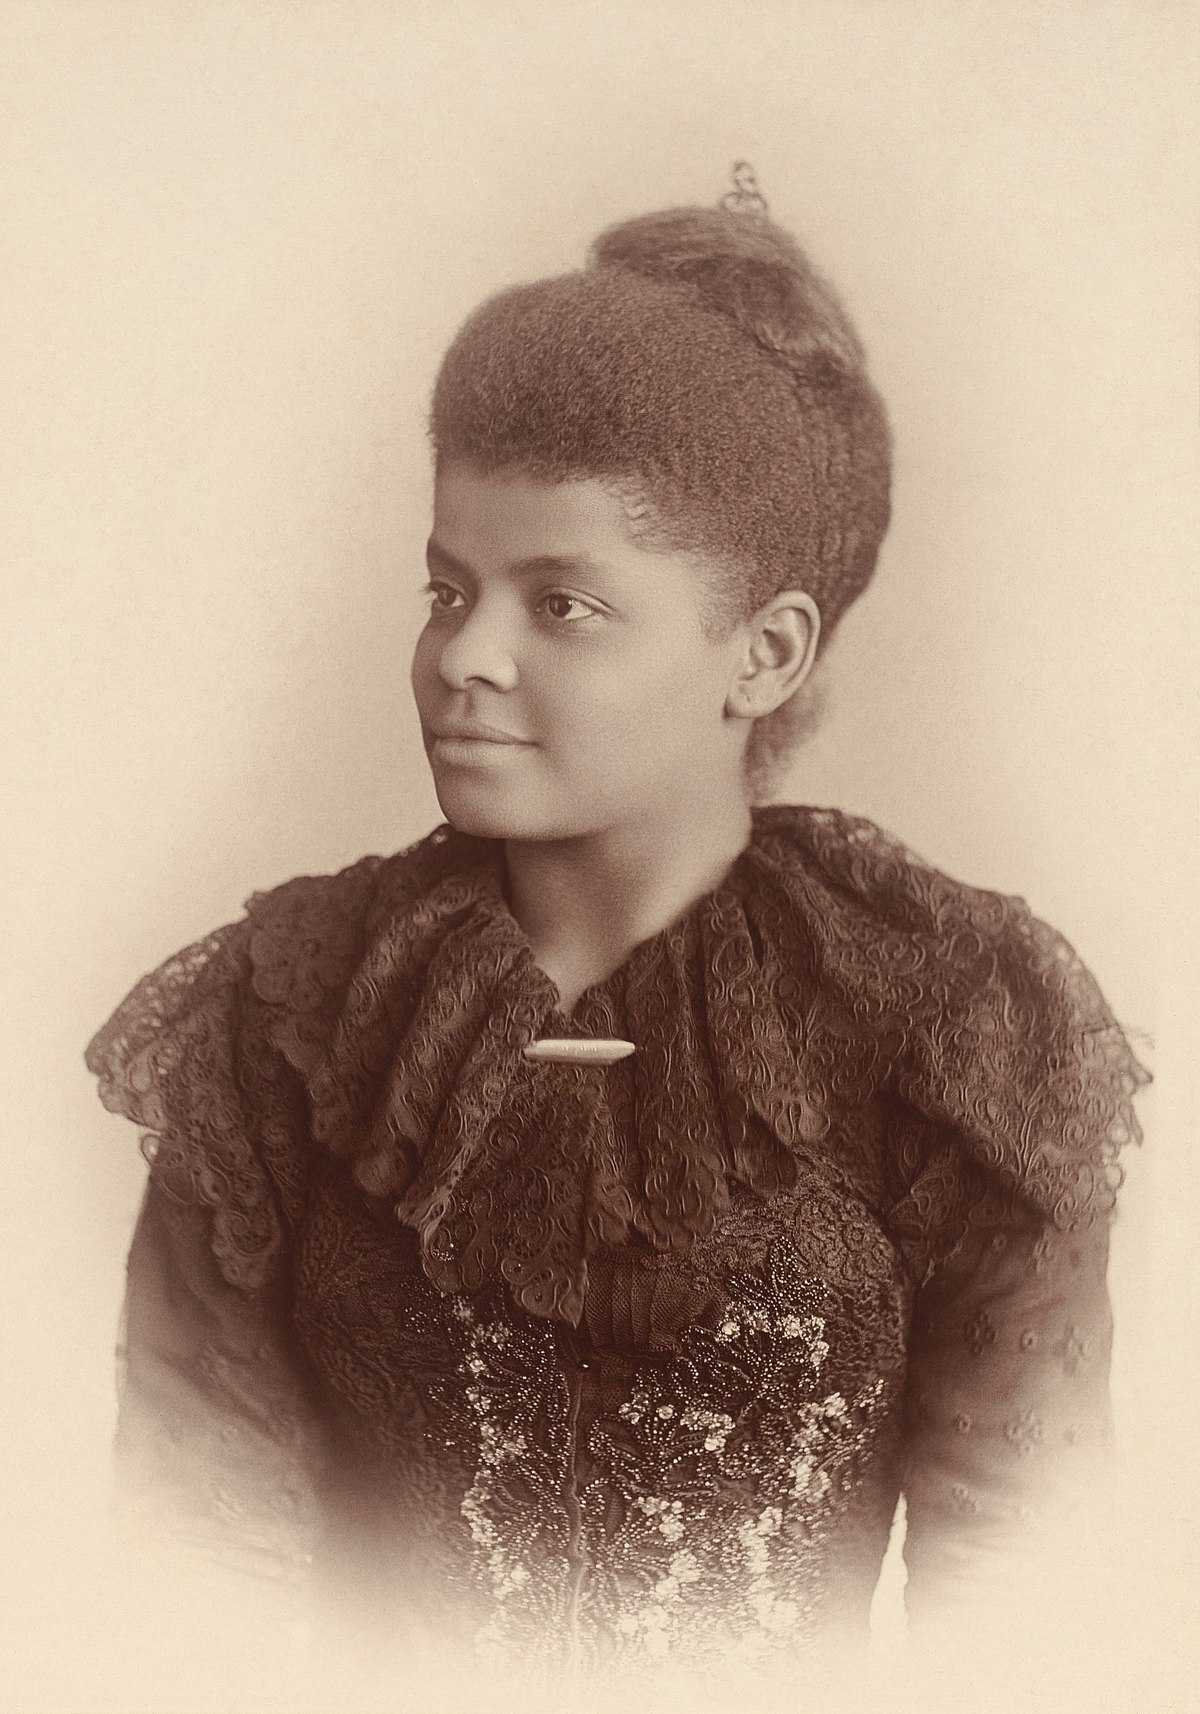
\includegraphics{ida1.jpg}

}

\caption{Ida B. Wells-Barnett}

}

\end{minipage}%
%
\begin{minipage}[t]{0.50\linewidth}

{\centering 

\raisebox{-\height}{

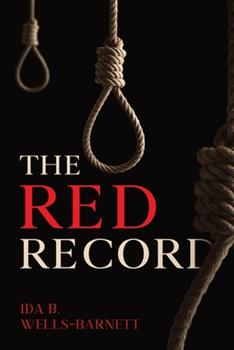
\includegraphics{ida2.jpg}

}

}

\end{minipage}%

\end{figure}

\begin{figure}

\begin{minipage}[t]{0.50\linewidth}

{\centering 

\raisebox{-\height}{

\includegraphics{dubois.jpg}

}

\caption{W. E. B. Du Bois}

}

\end{minipage}%
%
\begin{minipage}[t]{0.50\linewidth}

{\centering 

\raisebox{-\height}{

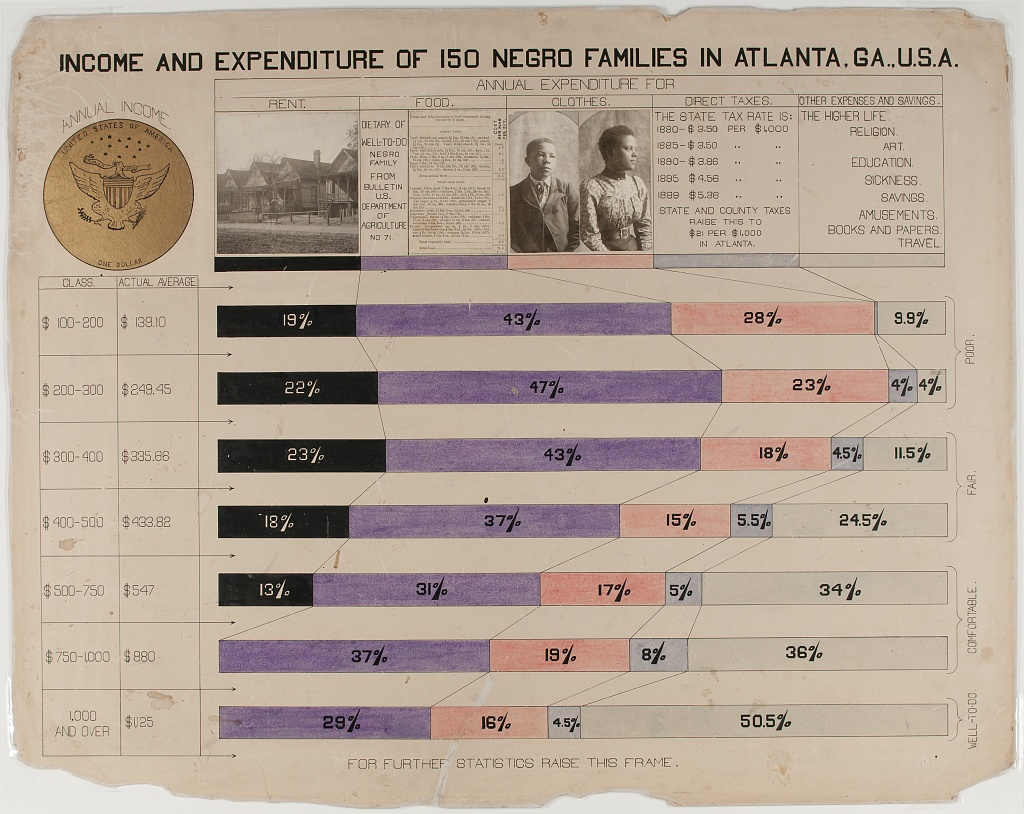
\includegraphics{w1d2a.jpg}

}

\caption{Income and Expenditure of 150 Negroe Families in Atlanta}

}

\end{minipage}%

\end{figure}

\begin{center}\rule{0.5\linewidth}{0.5pt}\end{center}

\hypertarget{exploration-of-journal-articles-and-citations-related-to-historical-of-inequity}{%
\subsubsection{Exploration of journal articles and citations related to
historical of
inequity}\label{exploration-of-journal-articles-and-citations-related-to-historical-of-inequity}}

Topic modeling research approach in STEM education journals

\begin{itemize}
\item
  Bibliometric analysis: who is citing who? who is discussing what?
\item
  Topic modeling: what are networks discussing?
\end{itemize}

\begin{center}\rule{0.5\linewidth}{0.5pt}\end{center}

Topic modeling research approach in STEM education journals

\begin{itemize}
\tightlist
\item
  What are the historical trends and patterns in the research on racism
  as reflected in journal articles?
\end{itemize}

\begin{figure}

{\centering 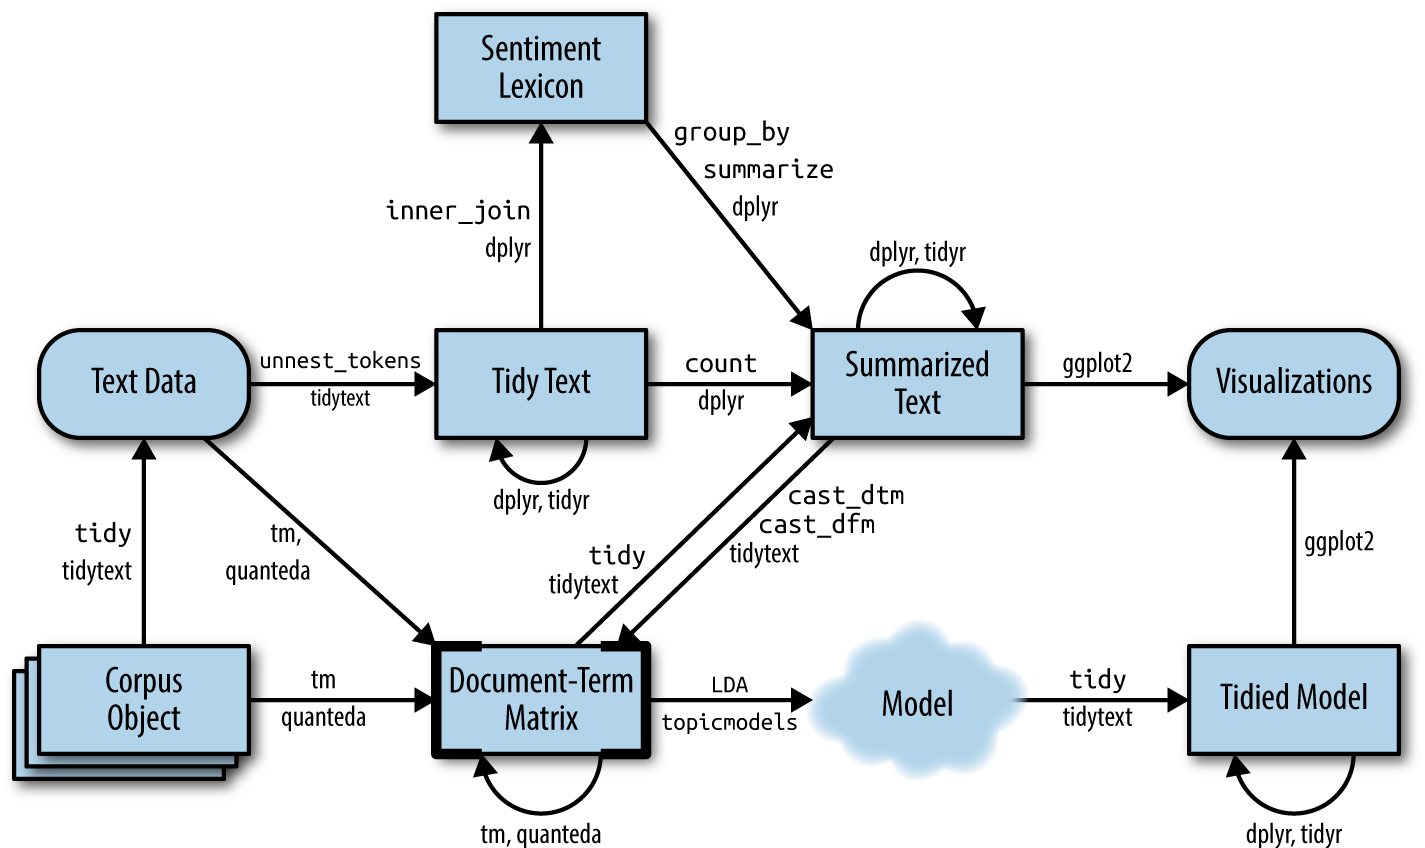
\includegraphics[width=0.5\textwidth,height=\textheight]{quanteda.png}

}

\caption{Topic modeling approach}

\end{figure}

\begin{center}\rule{0.5\linewidth}{0.5pt}\end{center}

\hypertarget{hypothesis-1-peaks-in-research-occur-within-some-key-historical-interval-t_1-t_2.}{%
\subsubsection{\texorpdfstring{Hypothesis 1: Peaks in research occur
within some key historical interval
\((t_1, t_2)\).}{Hypothesis 1: Peaks in research occur within some key historical interval (t\_1, t\_2).}}\label{hypothesis-1-peaks-in-research-occur-within-some-key-historical-interval-t_1-t_2.}}

\begin{figure}

{\centering 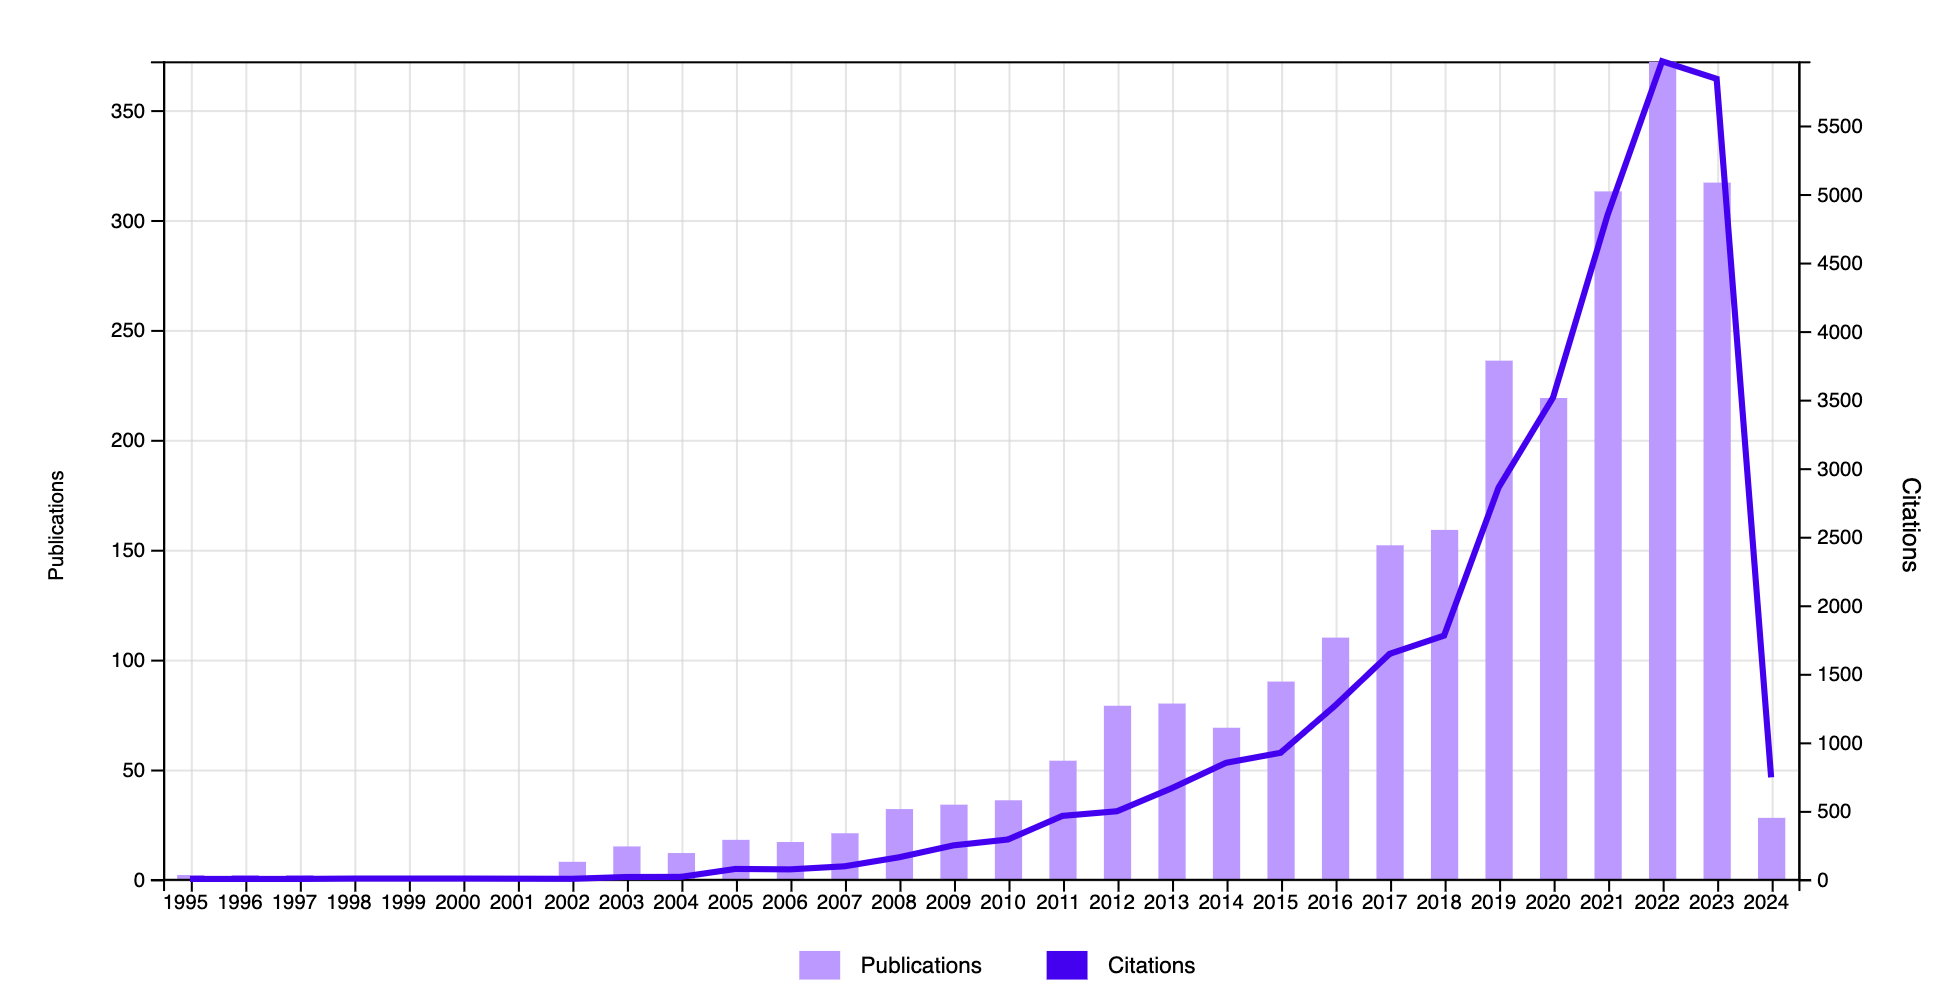
\includegraphics{report.png}

}

\caption{Publications and citations related to racism in STEM education}

\end{figure}

\begin{center}\rule{0.5\linewidth}{0.5pt}\end{center}

\hypertarget{hypothesis-2-these-intervals-are-lag-models-of-broader-system-searches-t_1-t_2.}{%
\subsubsection{\texorpdfstring{Hypothesis 2: These intervals are lag
models of broader system searches
\((t_1, t_2)\).}{Hypothesis 2: These intervals are lag models of broader system searches (t\_1, t\_2).}}\label{hypothesis-2-these-intervals-are-lag-models-of-broader-system-searches-t_1-t_2.}}

\begin{figure}

{\centering 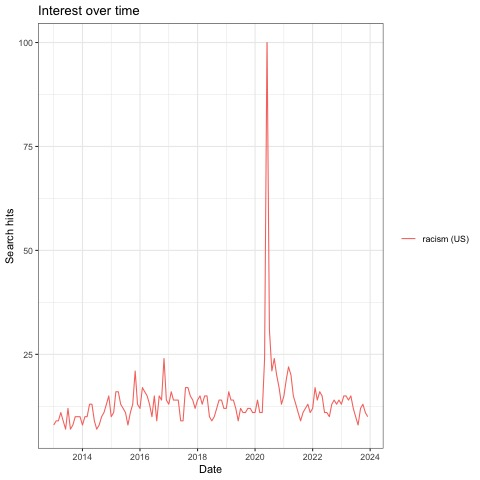
\includegraphics{racism-10year.jpeg}

}

\caption{Searches related to racism}

\end{figure}

\hypertarget{products}{%
\section{Products}\label{products}}

\begin{itemize}
\item
  \texttt{critstats} software package. An abstract introduction to
  critical statistics.
\item
  Playbook for educators to support and improve data science education.
\end{itemize}

\hypertarget{broad-implications}{%
\section{Broad Implications}\label{broad-implications}}

\begin{itemize}
\item
  K-12 teaching and learning

  \begin{itemize}
  \tightlist
  \item
    This also exposes students to a diversity of problems and methods to
    solve those problems.
  \end{itemize}
\item
  Computationally-focused research and training in higher education

  \begin{itemize}
  \tightlist
  \item
    Provides an equitable pathway and entry into ``high information,
    high density'' conversations.
  \end{itemize}
\item
  Industry and professional organizations
\end{itemize}



\end{document}
